\item \textbf{CodingJob: Um jogo sério para auxiliar nas disciplinas de Linguagem de Programação C}

A dissertação CodingJob \cite{costa2023condigjob} apresenta um jogo
sério que fornece um ambiente para prática dos conhecimentos da disciplina de
Linguagem de Programação I utilizando a linguagem C, não abrangindo nenhum
conceito de Estruturas de Dados.

Este é um jogo \emph{puzzle} que apresenta desafios de programação, simulando
um ambiente de trabalho, o objetivo do jogador é arrumar as secções de códigos
necessárias. Por se tratar de um simulador, o conteudo didático deste é
ensinado de forma explicita.

Por fim, identificou-se que o projeto analisado apresentou boa aceitação por
parte dos alunos participantes. O estudo também revelou que a narração exerce
um impacto mais significativo do que o inicialmente previsto na motivação dos
jogadores. Dessa forma, a construção de um enredo mais envolvente se mostra uma
característica fundamental a ser considerada em futuras melhorias, com o
objetivo de aumentar o engajamento dos usuários \cite{costa2023condigjob}.

\begin{figure}[H]
	\centering
	\caption{Captura de tela do jogo CodingJob}
	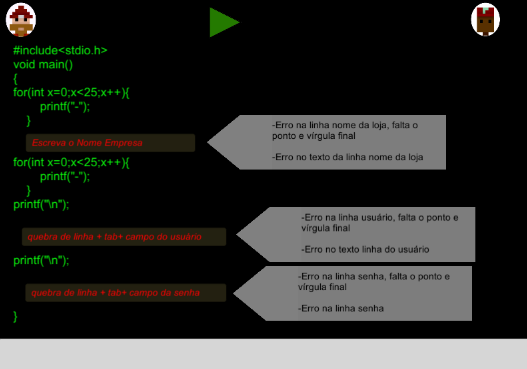
\includegraphics[width=0.8\textwidth]{images/codingjob.png}
	\legend{Fonte: \cite{costa2023condigjob}}
	\label{fig:codingjob}
\end{figure}

